
%%%%%%%%%%%%%%%%%%%%%%%%%%%%%%%%%%%%%%%%%%%%%%%%%%%%%%%%%%%%%%%%%%%%%%%%%%%% 

\chapter{Implementation Tools}%
\label{chapter:tools}


% introduction to implementation tools, unity game engine, vuforia for pose registration, urdf importer for unity, robot operating system, aruco marker for robot alignment, networking and protocols, conclusion
% The chapter will explore each tool in detail, providing a thorough explanation of its selection, integration within the project, as well as the contribution to the broader \ac{MR}-based \ac{HRC} framework.

\begin{introduction}
    To successfully integrate Human-Robot Collaboration and Mixed Reality technologies, a strategic selection of advanced software and hardware tools was essential. This chapter outlines the key technologies and platforms employed to build the Mixed Reality-based Digital Twin framework, enabling real-time, remote collaboration and bidirectional robot control. Developing such a system introduced challenges, including aligning physical and digital entities, achieving real-time data communication, and creating an immersive, user-friendly interface. Each tool presented in this chapter was selected for its specific role in overcoming these challenges and supporting the project’s objectives.
\end{introduction}

\section{UR10e Robot}

In order to start adressing the aforementioned challenges, a first effort has been made. THe robotic arm from Universal Robots, UR10e was used.

The UR10e model is one of Universal Robots' most advanced cobots, featuring a payload capacity of 12.5 kg, and a reach of 1300 mm, being designed to automate a wide range of tasks that typically require human input, such as assembly, packaging, and pick-and-place operations~\footnote{UR10e \url{https://www.universal-robots.com/products/ur10-robot/} Accessed: 2024-10-15}. UR10e's integrated force sensors and collision detection technologies allow to collaborate safely with humans in shared workspaces, making it ideal for \ac{HRC} scenarios. Besides, it offers significant flexibility in terms of programming and adaptability. Its console is intuitive and allows imported pre-programmed scripts, therefore being easily deployed across various industrial tasks with minimal programming experience required by the operator.

% \begin{figure}[h]
%     \centering
%     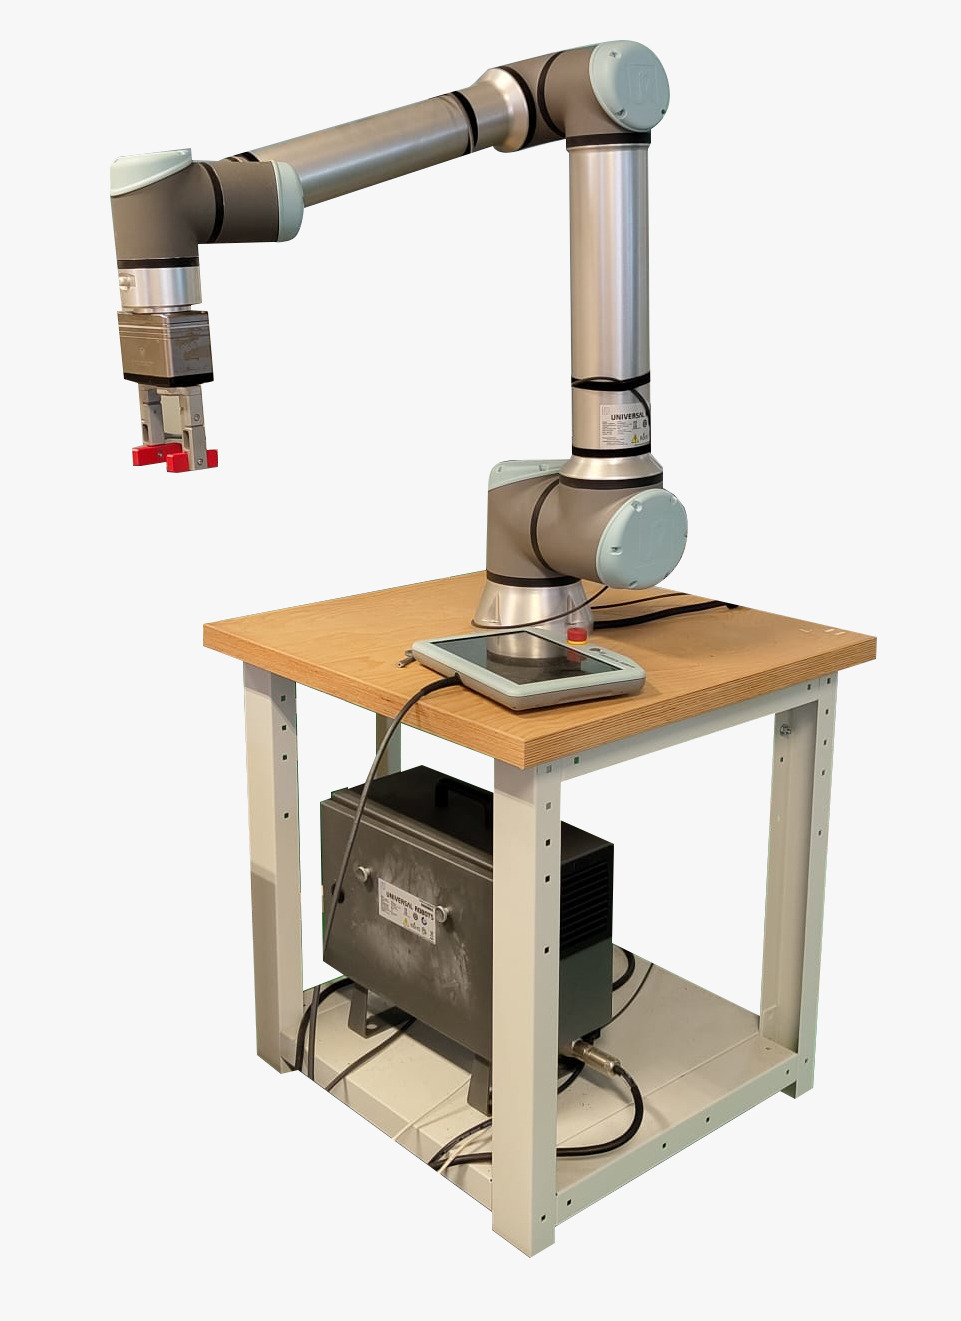
\includegraphics[width=0.4\linewidth]{figs/ur10e.jpeg}
%     \caption{UR10e Robot used in the robotics laboratory of IEETA, the Institute of Electronics and Informatics Engineering of Aveiro's University}
%     \label{f:ur10e_iris}
% \end{figure}

This robot, as the core physical entity in this human-robot collaborative system, serves as the dynamic agent for performing collaborative tasks, where its physical attributes were mirrored in an immersive digital environment, regarding the fundamental \ac{DT} concept.

\section{Simulation Environment}

Regarding the \ac{MR} application for \ac{HRC}, a simulation environment was essential to implement the \ac{DT} of the robotic system, design, 
visualize and interact with the developed features.

Unity, developed by Unity Technologies, was selected as the platform that would enable the development of this \ac{MR} environment. Originally designed for game development, Unity has evolved into a powerful tool for creating interactive 3D applications, including \ac{AR}, \ac{VR}, and \ac{MR}. Its robust architecture and versatility in rendering complex virtual environments make it an ideal choice for building a dynamic \ac{DT} of the UR10e robotic arm. This ability to seamlessly integrate external data sources, such as sensor inputs from real-world hardware, enables a high degree of interactivity and realism in the simulation.

Unity’s \ac{IDE} allows for rapid prototyping and iterative design of both the virtual space and the \ac{MR} user interface. Moreover, the engine's cross-platform compatibility supports a range of devices, including desktop systems and mobile platforms, and can handle real-time rendering of high-fidelity 3D models, essential for \ac{MR} applications. In addition, Unity’s robust asset management and scripting support, primarily through C\#, provide developers with the tools to easily simulate complex environments, manage interactive objects, and implement advanced functionality such as collision detection and user input handling.

Through the Unity-based simulation, users can, not only control the physical UR10e robot remotely, but also visualize real-world tasks in a digital, augmented environment, ensuring accurate synchronization between physical and virtual realms. These features enable a realistic and immersive experience for both on-site and remote members, aiming to improve the overall effectiveness of the \ac{HRC} system.

% \subsection{Digital Model Implementation of the Robot}

% Here, you can explain how the **Unity URDF Importer package** facilitated the import and management of the robot’s digital model, enabling the creation of a precise digital twin. This section should delve into the **Unity Robotics Hub**, explain why this package was selected, and describe how it contributed to the simulation of the UR10e’s movements and the development of bidirectional communication between the physical and digital environments.


% As introduced in section~\ref{section:Goals}, the primary objective of this dissertation is to explore and implement the concept of Human-Robot Collaboration (\ac{HRC}) by leveraging Mixed Reality (\ac{MR}) technologies. To achieve this goal, a comprehensive framework integrating hardware and software components is designed, facilitating remote collaboration in real-time. This chapter outlines the critical tools used in the implementation of the digital twin, as well as the hardware and software resources required for bidirectional robot control.



\section{Robot's Digital Model Implementation}
\label{section:digital-model}

A fundamental step in establishing a functional \ac{DT} is the accurate implementation of the robotic arm's digital model within the simulation environment. This setup is essential for ensuring that the \ac{DT}'s behavior mirrors the physical robot’s state in real time, paving the way for interactive manipulation.

The robot's \ac{URDF} model was integrated into the Unity simulation environment using the Unity Robotics Hub's \ac{URDF} Importer package~\footnote{\url{https://github.com/Unity-Technologies/Unity-Robotics-Hub} Accessed: 2024-02-02}. This package was instrumental in enabling an accurate digital representation of the UR10e’s physical structure, joints, and linkages, facilitating a precise recreation of its real-world dynamics in Unity.

The \textit{\ac{URDF} Importer} supported real-time simulation of the robot's kinematics providing a high level fidelity of physical behaviors. Additionally, it allowed the visualization and fine-tuning of physics properties to accurately reflect the robot's real-world dynamics. Essential for bilateral communication between virtual and physical models, the package also streamlined sensor data exchange from \ac{ROS}, enhancing the realism of simulations and optimizing development and testing processes.

\section{Pose Registration}
For the digital model to appear superimposed to the real robot, accurate alignment between the physical and digital models is critical. In this dissertation, Vuforia, a cutting-edge \ac{AR} software platform, was used to accomplish this alignment.

\subsection{Vuforia}
\label{section:marker-detection}

Vuforia Engine \ac{SDK}~\footnote{\url{https://developer.vuforia.com/downloads/SDK} Accessed: 2024-10-27}, an advanced \ac{AR} development platform that can be used within Unity platform, provides robust capabilities for object recognition and tracking, making it integral to \ac{MR} applications. In this project, Vuforia's image-based tracking system was employed to align the digital model of the robot with its physical counterpart.

\subsection{Marker Detection}

To ensure this precise spatial alignment between the digital and physical elements within the \ac{MR} environment, an ArUco marker~\footnote{\url{https://chev.me/arucogen/} Accessed: 2024-10-27} was placed next to the physical robot in the robotics laboratory of IEETA, as shown in Figure \ref{f:ur10e_iris} . This positioning is illustrated within the \ac{MR} simulation in Figure \ref{f:aruco_marker}, where the marker is positioned relative to the robot digital model. 

\begin{figure}[h]
    \centering
    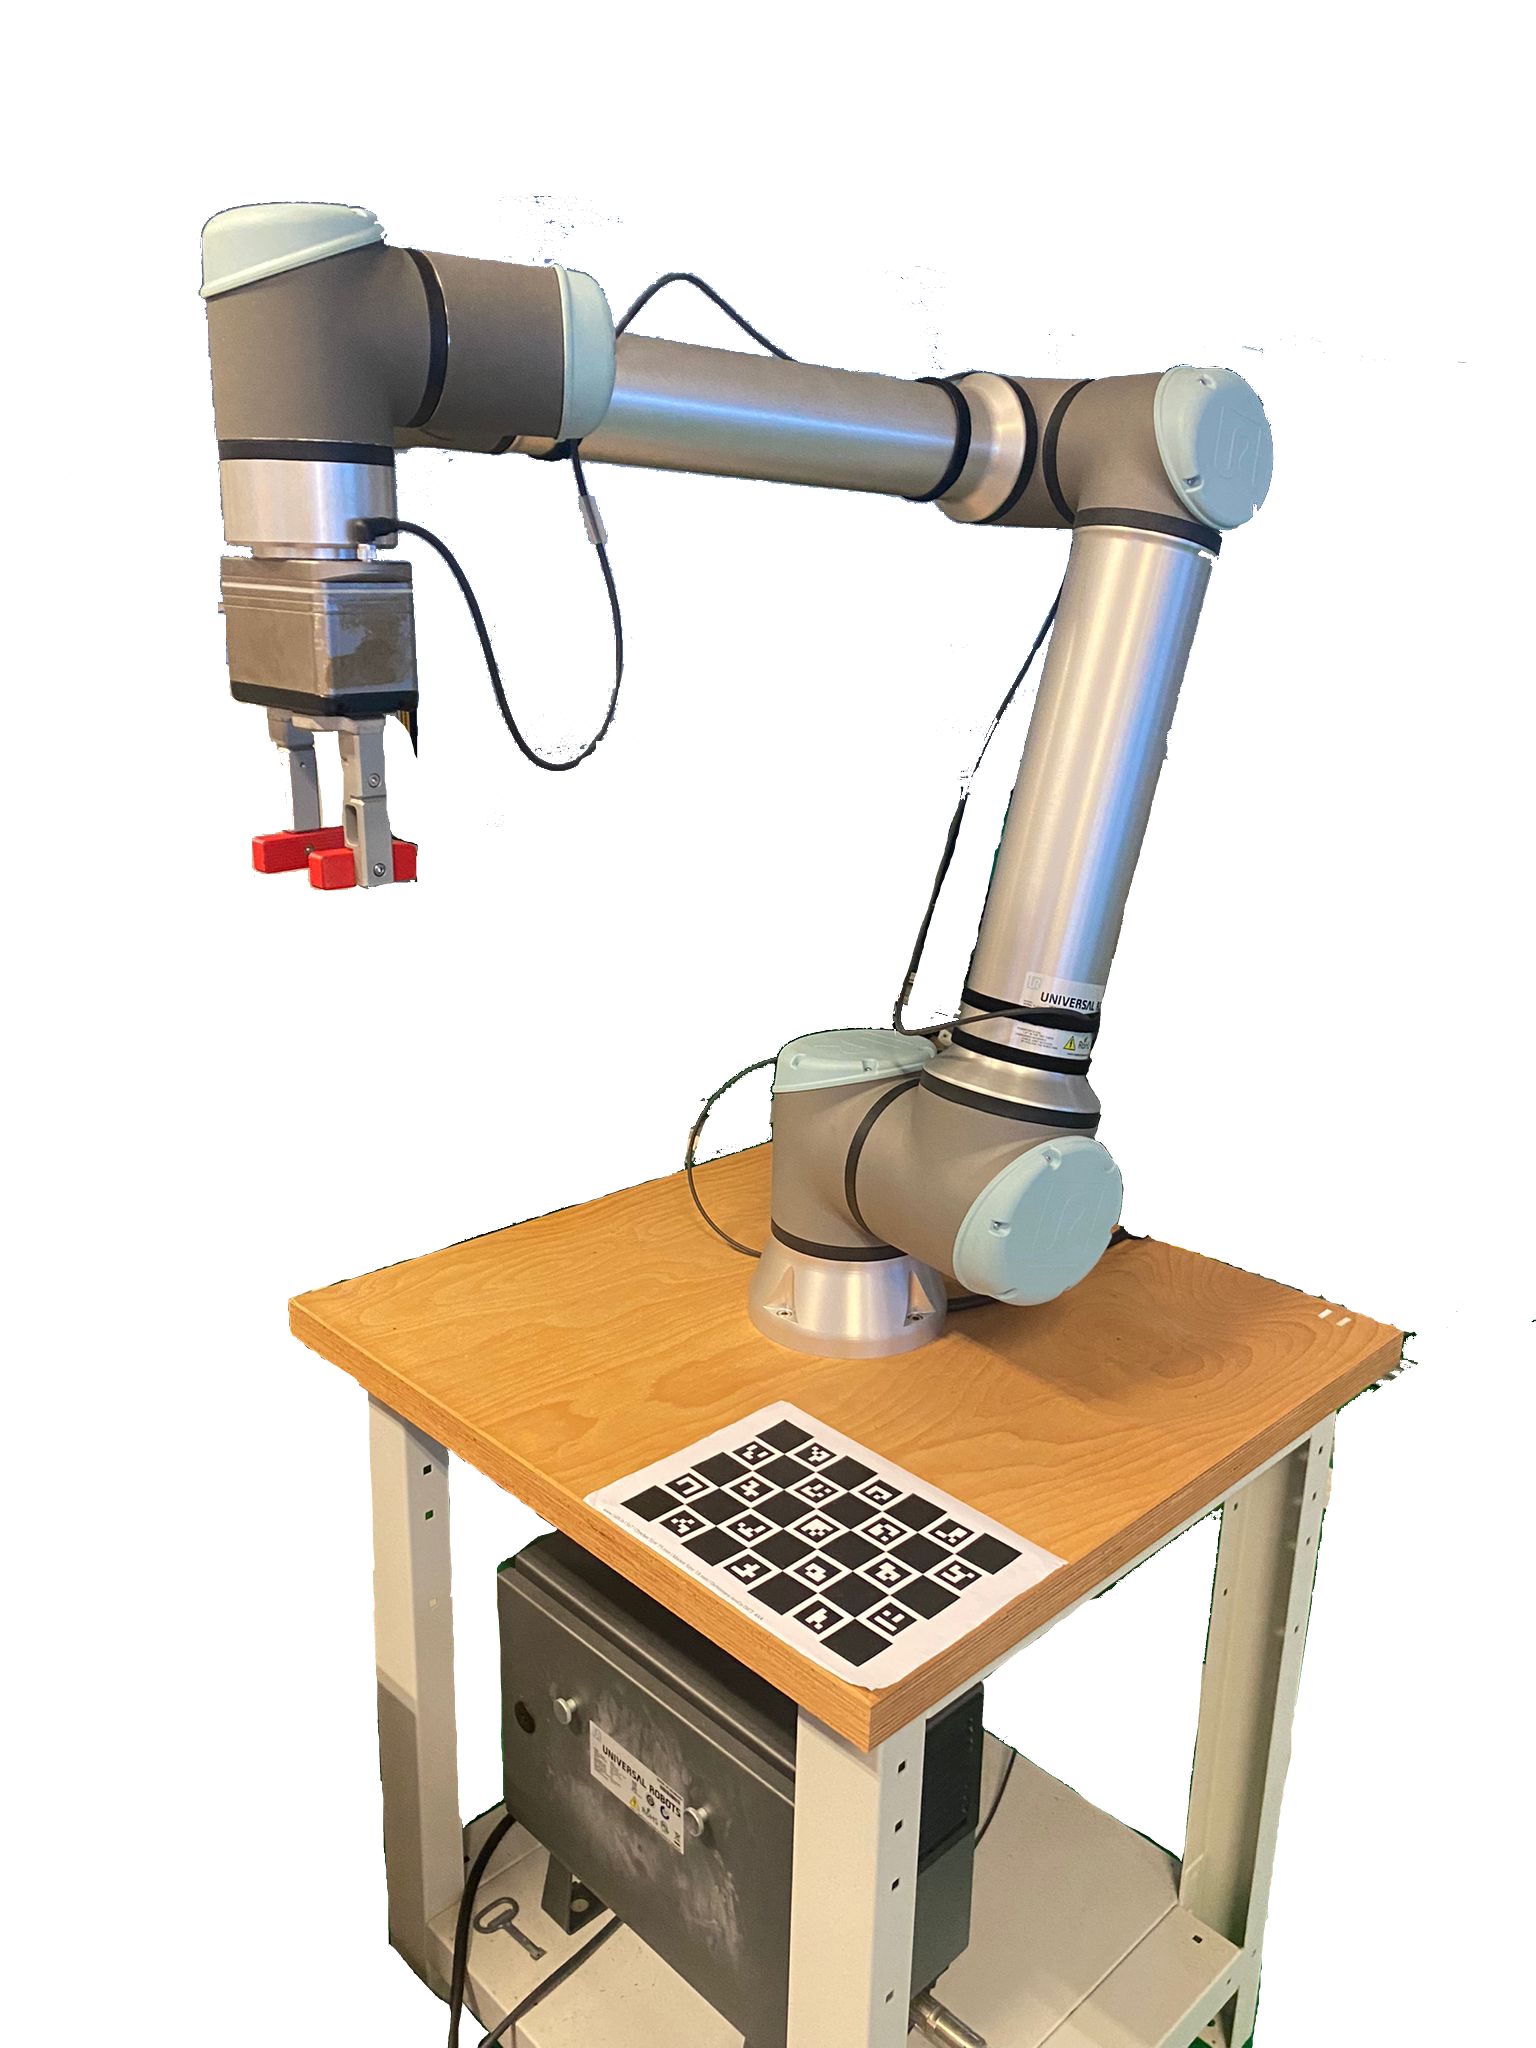
\includegraphics[width=0.35\linewidth]{figs/robot-marker.png}
    \caption{UR10e Robot and the marker used to align the digital model in the robotics laboratory of IEETA, the Institute of Electronics and Informatics Engineering of Aveiro's University}
    \label{f:ur10e_iris}
\end{figure}

To properly visualize the environment, the Logitech c922 camera, shown in Figure \ref{fig:camera-c922}, was used. It enables the robot digital model overlay to the physical robot, ensuring precise positioning and manipulation of the \ac{DT} in the \ac{MR} space.

\begin{figure}[h]
    \centering
    \begin{subfigure}[b]{0.45\textwidth}
    \centering
    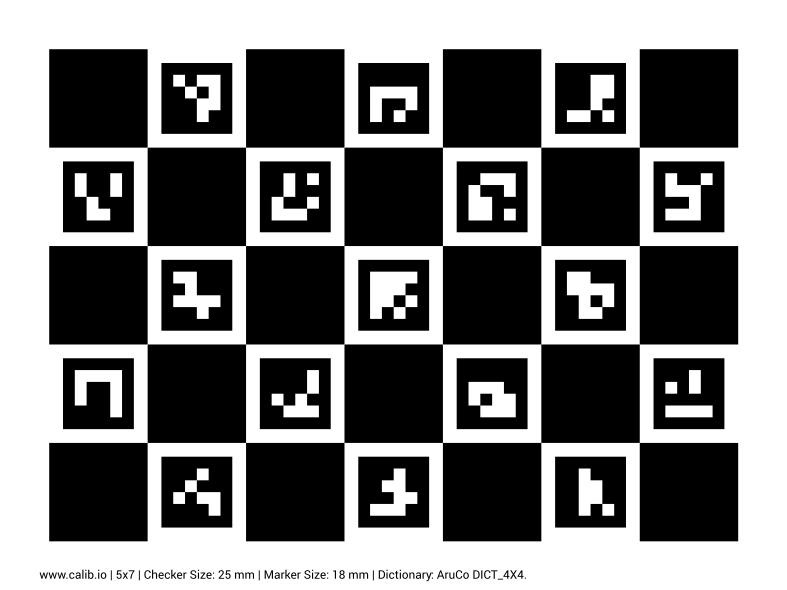
\includegraphics[width=0.7\textwidth]{figs/calib_io_charuco_200x150_5x7_25_18_DICT_4X4.png}
    \caption{ArUco marker for alignment of the digital twin}
    \label{f:aruco_marker}
    \end{subfigure}
        \hfill
    \begin{subfigure}[b]{0.45\textwidth}
        \centering
        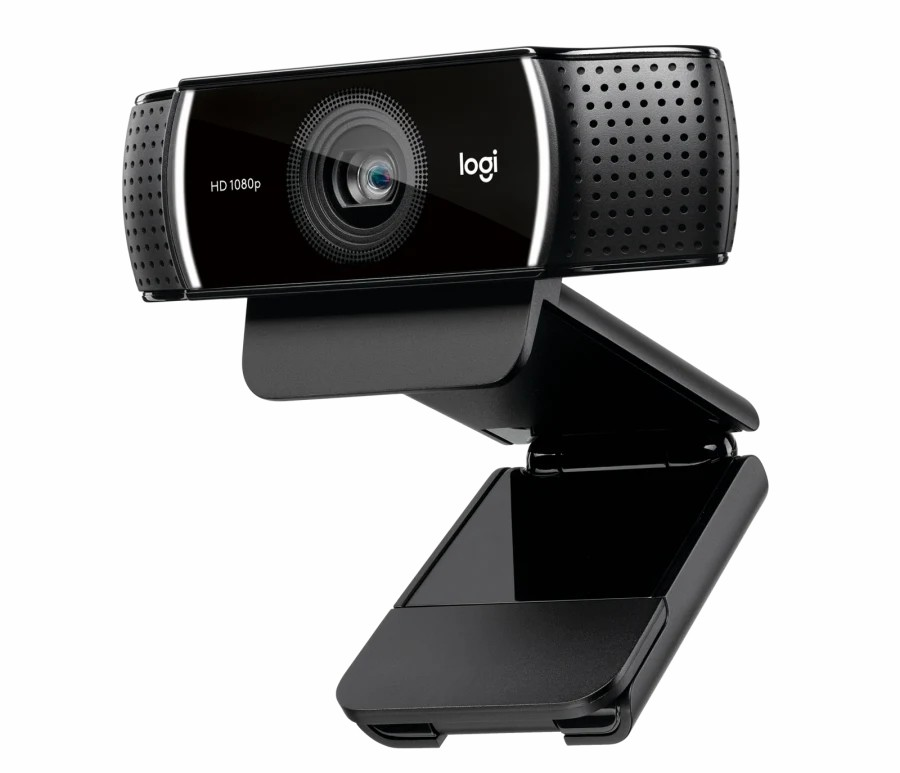
\includegraphics[width=0.7\linewidth]{figs/camera-c922.jpg}
        \caption{Logitech c922 camera used for marker detection}
        \label{fig:camera-c922}
    \end{subfigure}
    \caption{Marker and camera setup for digital and physical robot alignment}
\label{marker-camera}
\end{figure}

Figure \ref{f:ur10_marker_unity} displayes the digital robot model positioned realitve to the above described marker, within the Unity simulation environment.

\begin{figure}[h]
    \centering
    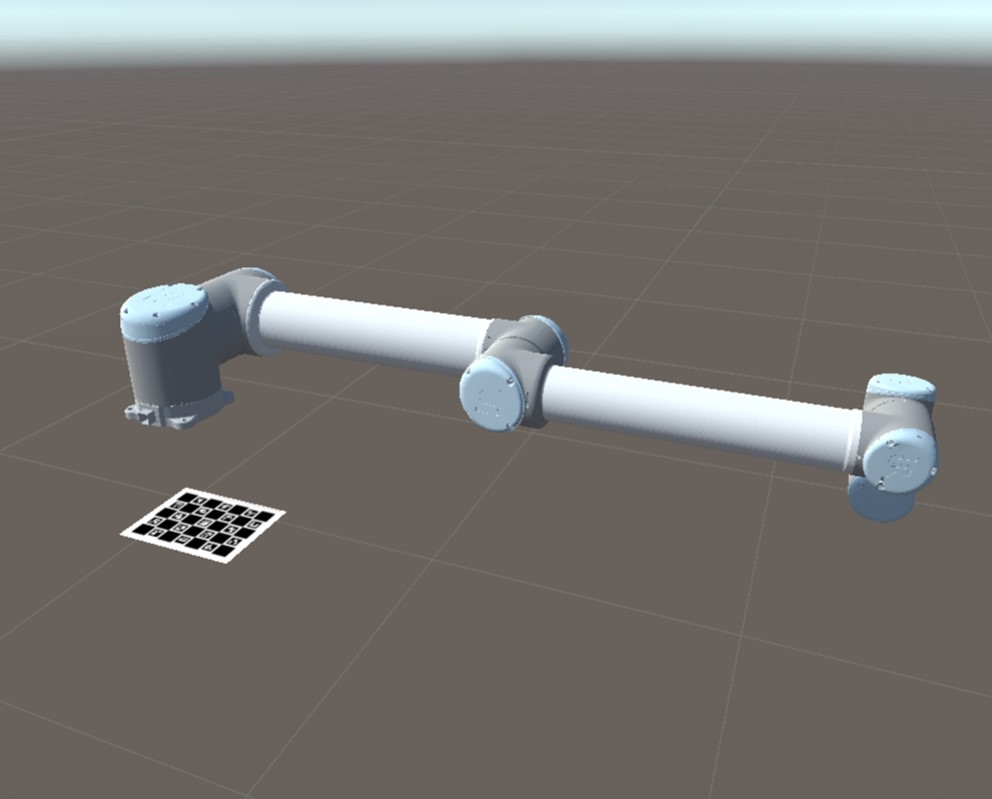
\includegraphics[width=0.6\textwidth]{figs/robot_marker_unity.jpg}
    \caption{Digital UR10 model aligned with ArUco marker in Unity}
    \label{f:ur10_marker_unity}
\end{figure}

\section{Bidirectional Communication}

After having the digital model correctly aligned with the physical robot, the next step consisted on establishing bidirectional communication between the Unity and the UR10e. This communication is essential to enable remote control of the physical entity through the \ac{DT}, as well as for synchronizing the robot's state between the real and virtual environments. This is relavant regarding the concept of \ac{DT} referred in \ref{sec:dt}, where bidirectional manipulation is essential when distinguishing between \ac{DT} and digital shadows. 

\ac{ROS}~\footnote{\url{https://www.ros.org/}, Acessed: 2024-10-27} is an open-source, flexible middleware framework that provides essential tools and libraries for developing complex robotic applications. Initially designed to support robotic research, it has evolved into a widely used framework in both academia and industry. By offering a standard architecture for robotic system integration, it allows different nodes to communicate and exchange data in real-time, supporting several functions such as sensor integration, data processing, and visualization.

It was suggested by the supervisors as the middleware software for facilitating real-time communication between the physical robot and the Unity \ac{MR} environment, since the UR10e robot from IRIS-LAB had already prior developed \ac{ROS} packages, such as \texttt{iris\_ur10e}~\footnote{\url{https://github.com/iris-ua/iris_ur10e}, Acessed: 2024-02-02} and \texttt{iris\_sami}~\footnote{\url{https://github.com/iris-ua/iris_sami}, Acessed: 2024-02-02}. These packages provide a comprehensive \ac{ROS} setup for controlling the UR10e robot, including trajectory planning, RViz visualization, and real-time robot manipulation. 
